\documentclass[a4paper,11pt,final]{article}
% Pour une impression recto verso, utilisez plutôt ce documentclass :
%\documentclass[a4paper,11pt,twoside,final]{article}

\usepackage[english,francais]{babel}
\usepackage[utf8]{inputenc}
\usepackage[T1]{fontenc}
\usepackage[pdftex]{graphicx}
\usepackage{setspace}
\usepackage[colorlinks,
            linkcolor=blue,
            anchorcolor=blue,
            urlcolor=blue,
            citecolor=blue
            ]{hyperref}
\usepackage[french]{varioref}
\usepackage{fancyhdr} % 添加页眉页脚
\usepackage{subfigure}
\usepackage{float}
\usepackage{textcomp}
\usepackage{multirow}
\usepackage{array}
\usepackage{longtable}

\newcommand{\reporttitle}{Rapport de Stage \\Année 2013-2014 \vspace{2ex}\\{\large Fouille de Donnée dans la domaine de télécommunication}}

\newcommand{\reportauthor}{Wenyi \textsc{wang}} % Auteur
\newcommand{\reportsubject}{Stage en Entreprise: Stage de fin d'étude} % Sujet
\newcommand{\HRule}{\rule{\linewidth}{0.5mm}}
\setlength{\parskip}{1ex} % Espace entre les paragraphes



\hypersetup{
    pdftitle={\reporttitle},%
    pdfauthor={\reportauthor},%
    pdfproducer={\reportauthor},%
    pdfsubject={\reportsubject},%
    pdfkeywords={rapport} {Fouille de donnée} {Mobile Communication} {LTE} {K-MEANS} {Apriori}
}

\pagestyle{fancy}
\lhead{}
\chead{Rapport de Stage}
\rhead{}
\lfoot{}
\cfoot{-\thepage-}
\rfoot{}
\setcounter{page}{3}
\begin{document}
  \pagestyle{empty}
  % Inspiré de http://en.wikibooks.org/wiki/LaTeX/Title_Creation

\begin{titlepage}

\begin{center}

\begin{minipage}[t]{0.48\textwidth}
  \begin{flushleft}
    
\includegraphics [width=30mm]{images/logo-univ.png} \\[0.3cm]
    \begin{spacing}{1.1}
      \textsc{\LARGE Université\\ Jean Monnet \\ \large spécialité Web intelligence}
    \end{spacing}
  \end{flushleft}
\end{minipage}
\begin{minipage}[t]{0.5\textwidth}
  \begin{flushright}
    
\includegraphics [width=30mm]{images/Tsinghua_University_Logo.png} \\[0.5cm]
    \textsc{\LARGE Tsinghuq University\\ \large Department of Electronic Engineering}
  \end{flushright}
\end{minipage}\\ [3.5ex]

\textsc{\Large \reportsubject}\\[0.1ex]
\HRule \\[0.4cm]
{\huge \bfseries \reporttitle}\\[0.2ex]
\HRule \\[10.5ex]

\begin{minipage}[t]{0.3\textwidth}
  \begin{flushleft} \large
    \emph{Auteur :}\\
    \reportauthor
  \end{flushleft}
\end{minipage}
\begin{minipage}[t]{0.6\textwidth}
  \begin{flushright} \large
    \emph{Tuteur de stage en entreprise:} \\
    Vice directeur de labo NGN:\\ yongfeng \textsc{huang} \\
    
    
    \emph{Tuteur de l'université:} \\
        Amaury \textsc{Habrard} \\
  \end{flushright}
\end{minipage}

\vfill
\vfill
{\large De 20 Février 2014 à 20 Juillet 2014}

\end{center}

\end{titlepage}

  \cleardoublepage % Dans le cas du recto verso, ajoute une page blanche si besoin
  %\pagenumbering{roman}
  \tableofcontents % Table des matières
  \thispagestyle{empty}
  \sloppy          % Justification moins stricte : des mots ne dépasseront pas des paragraphes
  \cleardoublepage 
  
  \thispagestyle{empty}
\section*{Remerciements}
\addcontentsline{toc}{section}{Remerciements}

Tout d’abord, je tiens à remercier Amaury Habrard et tous les enseignants de la Spécialité Web Intelligence de l’Université Jean Monnet, aussi les enseignants de Télécom Saint-Etienne et L'école nationale supérieure de Saint-Etienne, qui m’a aidé lors de ces deux années de étude.


Je remercie également M.Yongfeng \textsc{Huang} pour avoir accepter diriger cette stage, il m’a beaucoup conseillé, et les discussions que l’on a pu avoir se sont toujours révélées très intéressantes et instructives.


Je souhaite également adresser mes remerciement à Zheng \textsc{Yang}, Lindong \textsc{Wei} et xian \textsc{wu} ainsi que tout les membres du laboratoire de Next generation Network( \textbf{NGN} ) pour m’avoir soutenu, encouragé et conseillé tout au long de ce stage.


Je tiens à montrer tout ma gratitude envers toutes les personnes qui ont pu m’aider, m’encourager, me soutenir, me remotiver pendant ces années de travail.
  \cleardoublepage
  
  \pagestyle{fancy}  
  \pagenumbering{arabic}
  
%\addcontentsline{toc}{section}{Introduction} % Ajout dans la table des matières
\section{Résumé} 

Pendant ces quatre mois de stage, notre groupe de recherche travaille avec les employés de \textsc{cmcc} ( China Mobile Communications Corporation ) . Le objectif du sujet est: utilise les technique de Fouille de données, étude les données fournir par CMCC, et trouve les relation entre les données et les défaut du système 4G. Nous avons fait plusieurs tentatives pour trouver les résultats, et on a utilise différents logiciel, j'ai utilisé le R, et mon collègue utilise Mathlab, nous avons utilisé plusieurs algorithme (Clusterring, PCA, Association rules, Ajustement). Mais à la fin,  nous avons trouvé que à cause des défaut dans la système d'acquisition, les données ne sont pas correct, et nous ne pouvons pas trouver le résultat comme prévu. Mais les recherches que nous avons fait peut faites-leur savoir comment utilise les technique de fouille de donnée dans la domaine de télécommunication.

\section{Introduction} 
 
Le 3 avril 1973, M. Mation \textsc{cooper} le directeur général de la division communication de Motorola, à effectuer un appel téléphonique à Joel \textsc{engel}, son rival et néanmoins confrère chez \textsf{Belle Labs}. c'est la premier appel téléphonique en extérieur, L'idée du téléphone portable devient une réalité. 

depuis ce jour, le technique développé très rapidement. dans les 20 dernières années, il y a déjà quatre génération des standards pour la téléphonie mobile, non seulement nous pouvons appeler les autres, les nouvelles technologies et les Smart-phones nous permettons aussi envoyer les message, surfer l'Internet, utiliser le service RTSP(Real Timide Streaming Protocol), et le service VoIP (Voice over Internet Protocole),etc.. les services de communication téléphonique sont devenus un outil très important dans notre vie.
 
 \subsection{Introduction du CMCC}
 
Fondé en 3 Septembre 1997, après le regroupement de opérateur des télécommunications en 2008, \textsc{China Mobile Communications Corporation} (\textsf{CMCC})\ref{Fig.sub.1} est devenu un de trois opérateur des télécommunications en Chine (deux autres sont \textsf{China Unicom Co., Ltd.} et \textsf{China Telecom}). Après plusieurs années de développement, il a construit le plus grand réseau de communications mobiles dans le monde, possède la plus grande base d'utilisateurs dans le monde\ref{Fig.sub.2}. En 2013, CMCC a 767 million utilisateurs, 630,2 billion \textyen \qquad de revenu, 121,7 billions \textyen de revenus net, effectif 197,030.
\begin{figure}[H]
	\flushleft
	\subfigure[Logo de China Mobile]{
		\label{Fig.sub.1}
		
\includegraphics[width=1.8in]{images/China_Mobile_2013.png}}\hfill
	\hspace{1in}
%\flushright
	\subfigure[Reseau télécommunication]{
		\label{Fig.sub.2}
		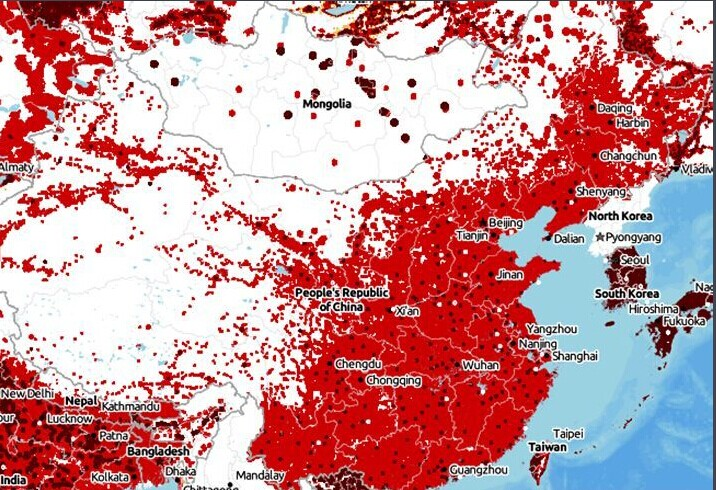
\includegraphics[width=2.0in]{images/reseau.jpg}}
	\caption{CMCC} 
\end{figure}

\subsection{La crise de CMCC}
Mais en même temps, le taux de croissance des nouveaux utilisateur décline de 22,5 \% (2006) à moins de 5\% 2013 \ref{tauxdecroissance}. Et dans la premier 3 mois, l'entreprise une fois considérés comme la plus rentable de Chine, le taux de croissance des revenu net est 0,3\%.

      \begin{figure}[H]
          \centering
          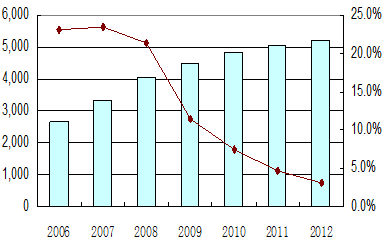
\includegraphics[width=3in]{images/1.png}
          \caption{le taux de croissance est décliner}
          \label{tauxdecroissance}
      \end{figure}
Opérateur des télécommunications Vodafone a fait un étude après il déployé un réseau 3G(\textsf{the third generation of mobile phone mobile communication technology standards}). Comme le réseau 3G permettant des débits (de 2 à 42 Mb/s définis par la dernière génération des réseaux) qui sont bien plus rapides que la génération précédente, par exemple le GSM. Les utilisateur utilisent bien plus souvent le service internet\ref{vodafone1}. Comme ils utilisent plus du service internet, le data ARPU (Average Revenue Per User) augment, mais le voix ARPU décline plus rapide que la montant de data ARPU\ref{vodafone2}. 
 \begin{figure}[H]
 	\flushleft
 	 	\subfigure[Downlink Data Traffic in 2G/3G Network]{
 	 	\label{vodafone1}
 	 	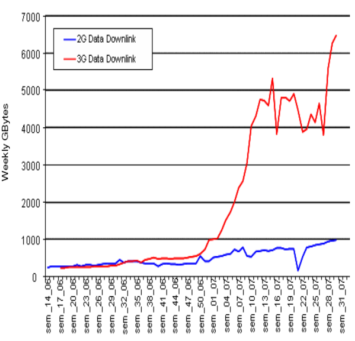
\includegraphics[width=2.0in]{images/4.png}}\hfill
 	\hspace{1in}	 
 	\subfigure[étude de Vodafone]{
 		\label{vodafone2}
 		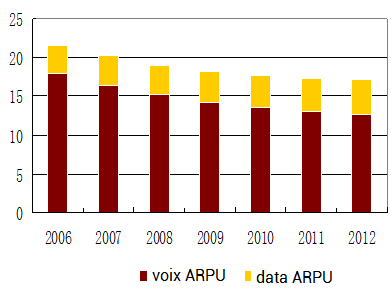
\includegraphics[width=1.8in]{images/2.png}}
 	\caption{Vodafone} 
 \end{figure}
 
Mais l'étude de Orange nous montre que si nous pouvons fournir des nouveaux technologies qui a plus haute débit, les utilisateur utiliseront plus souvent le service data.  \ref{traficparpersonne}
  \begin{figure}[H]
   \centering
   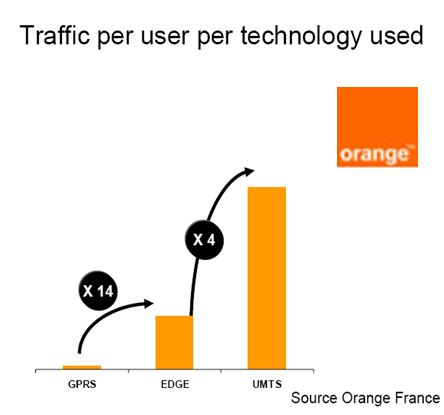
\includegraphics[width=3in]{images/orange.JPG}
   \caption{trafic par personne }
   \label{traficparpersonne}
  \end{figure}
 Des études nous montre nouveaux technologie (comme LTE) peut diminue le prix de revient, qui peut assurer le profit de l'opérateur. Mais déployé les nouveaux matériel coût très cher, en 2009, CMCC dépenser 30 billions \textyen en construit les station pour réseau 3G, et à 2014, CMCC a construit 1,5 million stations, à la fin de cet année, il y aura 1,8 million stations, parmi ces station, il y aura 500 mille stations TD-LTE. En ajoutant des équipement 4G, il peut être mis à niveau un station de 3G à 4G. Donc déployé le réseau 4G n'est pas trop cher, selon l'expérience précédente (de 2G à 3G), les utilisateurs iront utiliser plus le service internet, qui peut assurer le profit de l'entreprise.
      \begin{figure}[H]
          \centering
          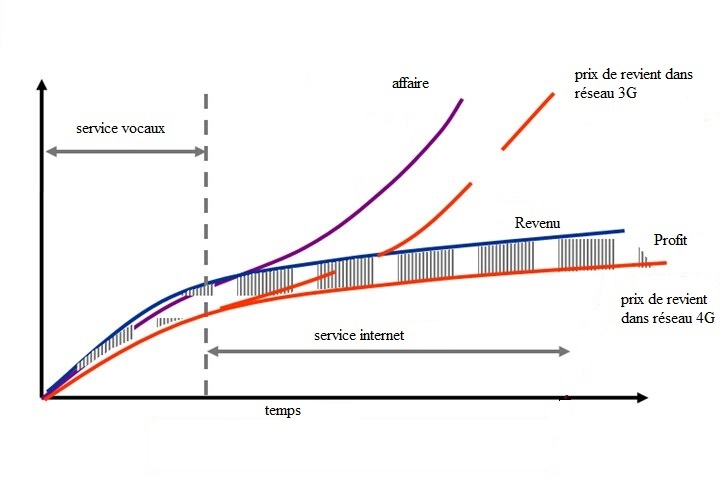
\includegraphics[width=3in]{images/why4G.jpg}
          \caption{4G est plus rentable}
          \label{why4G}
      \end{figure}
  \subsection{L'optimisation du réseau}
A part de la évolution des technologies. Un grand enjeu pour les opérateurs est: l'optimisation du réseau télécommunication. Le réseau de communication mobile est très dynamique, la répartition de la densité du trafic est inégale, fréquence très limité, etc. La configuration du réseau état toujours sous-optimal, et la perception de l'utilisateur n'est pas très bien. Donc tous les opérateurs doivent toujours reconfigurer/optimiser/maintien les paramètre du réseau.
  
Les opérateurs peuvent percevoir les données sur Internet, et utilisent ces informations pour trouver les défauts du système, peut aide l'entreprise optimiser le système.

Mais la optimisation du réseau télécommunication est difficile parce-que: Les technologies d'optimisation de réseau concerné: La technologie de commutation, la technologie sans fil, la configuration et commutation de la fréquence, la signalisation système, l'analyse de trafic, etc. c'est un travail difficile, exiger une meilleure aptitude des employés.  

Actuellement, l'optimisation du réseau dépend principalement à la expérience du personnel. Mais des fois les expériences ne sont pas correct. Par exemple, Si l'entreprise besoin de savoir le congestionné d'un station, il faut envoyer les employé avec des équipement pendant les périodes de pointe, mais on ne sait pas si les résultats sont correct \ref{meseau}.  En outre, souvent un seul type de  donnée ont utilise pour l'analyse et la comparaison pour optimiser les réseau, plutôt que de trouver un solution d'optimisation basées sur toutes les données liées au réseau (telles que les données statistique de trafic, les données d'essai, etc). Et en raison de l'énorme quantité de données, c'est difficile de traite en temps opportun. il est évident que ce méthode est défectueux. Les défauts du système provoque la satisfaction des utilisateurs inférieure, ce qui a conduit à multiplier.
      \begin{figure}[H]
          \centering
          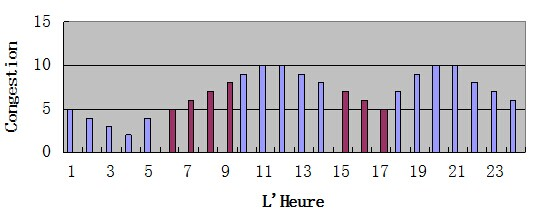
\includegraphics[width=3in]{images/meseau.jpg}
          \caption{Mesure la congestionné d'un station}
          \label{meseau}
      \end{figure}
      
Face à des problèmes complexes, les grands entreprises commence utilise les techniques de Fouille de données. Ce technique peut aide l'entreprise faire les décision plus vite et plus précis.

De ce faire, en Juillet 2013, CMCC a lancé ce projet avec quatre laboratoires dans trois université, ils sont
 \href{http://www.tsinghua.edu.cn/publish/newthuen/index.html}{Tsinghua University}, \href{http://en.sdu.edu.cn/}{Shandong University} et \href{http://www.oice.uestc.edu.cn/en/}{University of Electronic Science and Technology of China}. Le projet inclure trois partiel: Fouille de données, gérés le Clound plateforme et modélisation de l'information dans le système.
 

  \subsection{Introduction du laboratoire}
 De 20 Avril 2014 à 20 Juillet 2014, je fait mon stage chez \href{http://203.91.121.76/joomla/}{laboratoire of Next Generation Network Technology \& Application} \textsf{( NGN )} \ref{Logo NGN}. C'est d'un subordonné de \href{http://www.ee.tsinghua.edu.cn/publish/eeen/3776/index.html}{Research Institute of Network And Human-Machine Speech Comunication}, Département Ingénierie électronique, Tsinghua University. Le laboratoire se trouve dans la ROHM bâtiment.
  \begin{figure}[H]
      \centering
      
\includegraphics[width=3in]{images/NGN.jpg}
      \caption{Logo NGN}
      \label{Logo NGN}
  \end{figure}
Le principaux axes de recherche sont Théorie des réseaux, Architecture de l'Internet, Traitement de l'information Internet, La recherche dans le domaine de la sécurité Internet, Sentiment analyse, Information hiding, etc.

 Mon tuteur professionnel est \href{http://203.91.121.76/joomla/index.php/staff/teacher/83-huangyongfeng}{M. Yongfeng \textsc{huang}}, vice-directeur de la laboratoire NGN. Dans le laboratoire, il y a cinq groupe, chaque groupe a un docteur et son sujet. dans notre groupes, il y a trois personnes, un étudiant de premier année docteur, un étudiant de M1, et une étudiante de Licence troisième année. On utilise R et Rstudio, et Hadoop aussi.
 
 \subsection{Objectif du projet}
Dans cet article, nous avons d'abord présente le réseau communication mobile, ensuite je vais décrire l'état de l'optimisation du réseau. Enfin je présente la mise en place de notre programme de recherche. 
  \cleardoublepage
  
  % !TeX spellcheck = fr-moderne
\section{Introduction de l'industrie de la télécommunication}
\subsection{L'evolution des normes de téléphonie mobile}
Depuis 1984, il y a déjà plusieurs standards ont été utilisé par les opérateur dans le monde entier. Voici un tableau de différentes standards mobile en Europe et ses paramétrés \ref{tbl:GMIE}. 
\begin{table}[H]
\begin{tabular}{|p{2cm}|p{2cm}|p{2cm}|p{4cm}|}
	\hline
	Génération&Acronyme&Description&Débit\\
	\hline
	1G		&Radiocom 2000	&Échanges de type voix uniquement&analogique\\
	\hline
	\hline
	2G		&GSM			&Échanges de type voix uniquement	&9,05 kbps\\
	\hline
	2,5G	&GPRS			&Échange de données sauf voix		&171,2 kbps / 50 kbps / 17,9 kbps\\
	\hline
	\hline
	3G		&UMTS			&Voix + données						&144 kbps rurale, 384 kbps urbaine, 1,9 Mbps point fixe / -\\
	\hline
	3.5G ou 3G+ ou H&HSPA	&Évolution de l'UMTS				&14,4 Mbps / 3,6 Mbps / -\\
	\hline
	\hline
	4G		&LTE			&Long Term Evolution (Données)				&150 Mbps / 40 Mbps / -\\
	\hline
	4G		&LTE-Advanced	&Long Term Evolution Advanced (Données+voix)		&1 Gbps à l'arrêt, 100 Mbps en mouvement / - / -\\
	\hline
\end{tabular}
\caption{Les différentes générations de téléphonie mobile en Europe}
 \label{tbl:GMIE}
\end{table}

\subsubsection{La premier génération}
En télécommunication, \textsf{1G} est la premier génération des standards pour la téléphonie mobile, il s'agit de la première apparition du réseaux de téléphonie mobile, 1G sont des réseaux analogiques, peut échanges de type voix uniquement.
\subsubsection{La deuxième génération}
\textsf{2G}, la technologie de téléphonie sans fil de deuxième génération, la différence entre le réseaux 1G et 2G est: le signaux radio sur les réseaux 1G sont analogiques, et celle de 2G sont numériques.

Systèmes 2G ont été significativement plus efficaces du spectre permettant de bien plus grand taux de pénétration du téléphone mobile, en plus les données vocales numériques peuvent être compressées et multiplexées beaucoup plus efficacement que les codages de la voix analogique grâce à l'utilisation de codecs différents, ce qui permet plus d'appels à transmettre dans la même quantité de bande passante radio. Et 2G présenté premier foi les services de données pour mobile. Les Technologie 2G permettent les divers réseaux de téléphonie mobile de utiliser des services tels que le SMS et MMS. Tous les message de texte envoyés au delà de 2G sont chiffrés numériquement, ce qui permet le transfert de données de telle sorte que seul le destinataire peut recevoir et lire.   

Réseaux 2G ont été construits principalement pour les services téléphoniques et de transmission de données lent (défini dans les documents de spécifications IMT-2000).

Réseaux \textsf{2,5G}, on le qualifie souvent de le General packet Radio Service ou GPRS, est une norme pour la téléphonie mobile dérivée du GSM et complémentaire de celui-ci, permettant un débit de données plus élevé. Le 2,5 indique que c'est une technologie à mi-chemin entre le GSM (deuxième génération) et l'UMTS (troisième génération). Le GPRS est une extension du protocole GSM : il ajoute par rapport à ce dernier la transmission par paquets. Cette méthode est plus adaptée à la transmission des données. En effet, les ressources ne sont allouées que lorsque des données sont échangées, contrairement au mode « circuit » en GSM où un circuit est établi – et les ressources associées – pour toute la durée de la communication. Le GPRS a ensuite évolué au début des années 2000 vers la norme \textsc{edge} également optimisée pour transférer des données et qui utilise les mêmes antennes et les mêmes fréquences radio.
\subsubsection{La troisième génération}
La troisième génération (3G) des normes de téléphonie mobile. Elle est représentée principalement par W-CDMAmm, CDMA2000, TD-SCDMA et WiMAX. Elle permettant des débits de 2 à 42 Mb/s qui sont bien plus rapides qu'avec la génération précédente. Grâce à l'utilisation des règles de classement de l'utilisateur, et les  bandes de fréquences supérieures rendant la capacité du réseau augmenter.

Dans les différentes standard  3G et ses prédécesseur, ils utilisent le domaine CS (Circuit Switch)  pour les services vocaux, et le domaine PS (Packet Switch) s'occupe des services de données \ref{Fig.3G.1}.
\subsubsection{La quatrième génération}
La quatrième génération des standards pour la téléphonie mobile, succédant à la 2G et la 3G, en théorie, elle permet de transmette de données à des débits supérieur à 100 Mb/s. 

Une des particularité de la 4G est sa EPC (Evolved Packet Core) est basé sur IP, et il n'y a plus de mode commuté (le 'Circuit Switched Domain' qui s'occupe le service vocaux dans les standard précédant), ce qui signifie que les services vocaux transmis sur l'internet \ref{Fig.3G.2}. 



\begin{figure}[H]
	\centering
	\subfigure[Réseau 3G et ses prédécesseur]{
		\label{Fig.3G.1}
		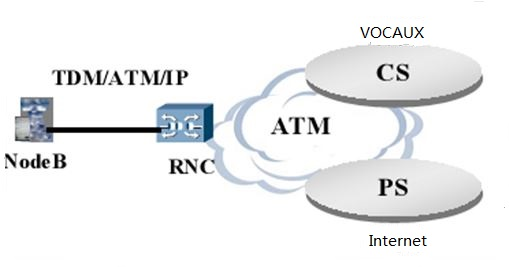
\includegraphics[width=3in]{images/3G2.JPG}}\hfill		
	\hspace{1in}
%\flushright
	\subfigure[Réseau 4G]{
		\label{Fig.3G.2}
		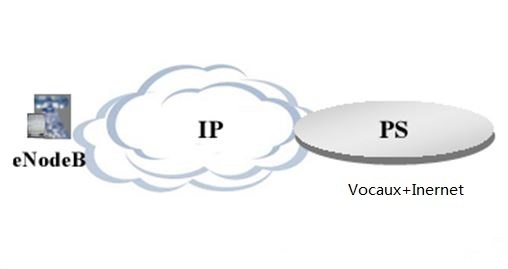
\includegraphics[width=3in]{images/4g.JPG}}
	\caption{Structure des réseaux} 
		\label{Fig.3G}
\end{figure}
Les avantages du réseau 4G sont:  plus haut débit, mieux utilisation de la bandes de fréquence, moins de délai (délai dans le panneau de l'utilisateur est inférieur que 5 ms, délai dans le panneau de commande est inférieur que 100 ms ), plus simple structure du réseau, moins de consommation d'énergie Terminal.

\subsection{Le réseau LTE}
Le LTE (Long Term Evolution) est l'evolution la plus récent des normes de CDMA 2000, TD-SCDMA, GSM. La norme LTE. La technologie LTE été considérée comme une norme de troisième génération '3.9G', et la 'vraie 4G', appelée LTE-Advanced été reconnu par l'UIT comme une technologie 4G en 2010. LTE a deux branche: LTE-FDD (Frequency-Division Duplex  Long Term Evolution)et LTE-TDD, (Time Division Duplex Long Term Evolution)les deux standards sont similaire, la différence entre les deux standard est moins de 15\% \ref{evolution}. En 2011-2012, les réseaux LTE-TDD sont commercialisés sous l'appellation 4G par CMCC un Chine.
      \begin{figure}[H]
          \centering
          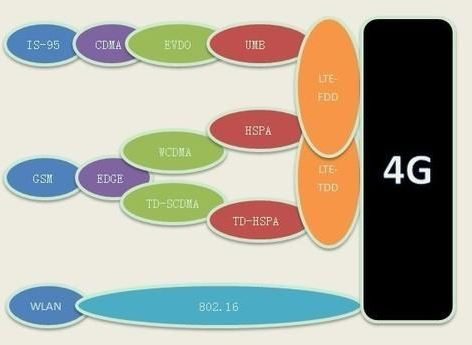
\includegraphics[width=4in]{images/evolution.JPG}
          \caption{l'evolution des standard}
          \label{evolution}
      \end{figure}
      
\subsubsection{La structure du réseau LTE}
Le réseau 4G contient 3 partie: UE( User Equipment);, eNodeB (les stations de base), EPC (Evolved Packet Core). EPC contient MME, S-GW, P-GW et HSS \ref{structure4G}  \ref{founction du chaque partie}. 
    
      \begin{figure}[H]
          \centering
          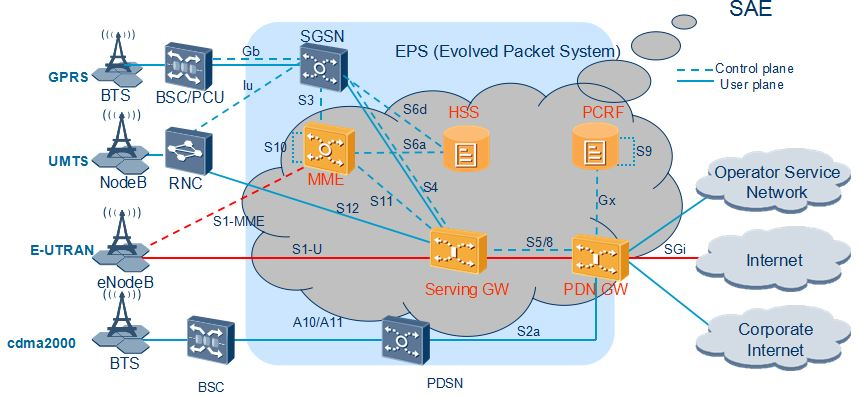
\includegraphics[width=5in]{images/enb2.jpg}
          \caption{la structure du réseau}
          \label{structure4G}
      \end{figure}
      
\begin{table}[H]
	\begin{tabular}{|>{\centering\arraybackslash}p{2cm}|>{\centering\arraybackslash}p{11 cm}|}
		\hline Part &                     Fonction\\
		\hline MME & 
			L'authentification des utilisateurs et la gestion des clés,  Cryptage de la couche NAS,  Gestion de la liste TA, Sélection P-GW ou S-GW \\ 
		\hline Service Gateway & Compression d'en-tête IP, Routage de paquets et la transmission, La commutation entre eNB, Facturation des utilisateurs porteur \\ 
		\hline PDN Gateway & L'allocation des adresses IP de UE, l'accès aux fonction de gestion de réseau externes, Facturation en service \\ 
		\hline HSS(Home Subscriber Service) & Stockée données de l'utilisateur associées au service \\ 
		\hline PCRF & Roaming \\ 
		\hline 
	\end{tabular} 
	\caption{la fonction du chaque partie}
	\label{founction du chaque partie}
\end{table}    

Entre deux \textsc{e-utran}, il y a l'interface X2, l'interface S-11 se trouve entre S-GW et MME, \textsc{e-utran} et S-GW échange les données par l'interface S1-U \ref{Fig.S1}et il échange les donnée par l'interface S1-AP avec MME \ref{Fig.S1}, MME et HSS utilise l'interface S6A, et l'interface S5/8 entre S-GW et P-GW, Gx entre PCRF et P-GW. En mettant des capteur en les interfaces, les opérateurs et les fournisseurs d'équipement peuvent collecter les données de signalisation, et utilisent ces informations pour trouver les défauts du système. 
      \begin{figure}[H]
          \centering
          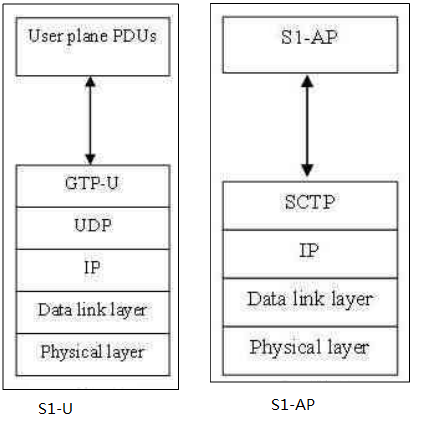
\includegraphics[width=2in]{images/S1-U.png}
          \caption{Interface S1}
          \label{Fig.S1}
      \end{figure}

\section{Introduction des données}
%\,\up{\cite{specifi}}
Après quelque semaines de négociation avec les employés de différents départements de la CMCC, ils nous ont fourni deux versions de données, et ses spécifications du format\cite{specifi}. Nous avons trouvé que CMCC n'a pas de accès direct aux données, et le fournisseur d'équipement a modifié le spécification fournir par CMCC, et il y a des erreurs dans les données fourni par les fournisseur d'équipement.

Ils nous ont envoyé $11$ dossiers, chaque dossier correspond à un service. les services sont 'rtsp', 'dns','mail', 'ftp', 'http-wap', 'mms', 'p2p', 'realtimecom', 'VoIP' et les données de signalisation entre \textsc{e-utran} et MME 'S1AP-NAS'\ref{dossier}. 
      \begin{figure}[H]
          \centering
          
\includegraphics[width=5in]{images/data.png}
          \caption{les dossiers de données}
          \label{dossier}
      \end{figure}
Et nous avons trouvé que pour les services comme 'VoIP' et 'RTSP', ils sont très peu de données \ref{table.nombre}. Donc nous avons décidé de utiliser le donnée du service 'HTTP'.

\begin{table}[H]
\centering
	\begin{tabular}{|>{\centering\arraybackslash}p{4 cm}|>{\centering\arraybackslash}p{4 cm}|}
	\hline \textsf{L'interface }& \textsf{Nombre de ligne} \\ 
	\hline S1-AP & $240$ \\ 
	\hline RTSP &$ 35$ \\ 
	\hline DNS  & $272562$ \\ 
	\hline Maill & $44$ \\ 
	\hline FTP &$ 71$ \\ 
	\hline HTTP-WAP & $50854$ \\ 
	\hline MMS & $193$ \\ 
	\hline P2P & $515$ \\ 
	\hline Realtimecom & $2082$ \\ 
	\hline S1U &$ 89759$ \\ 
	\hline VoIP & $28$ \\ 
	\hline 
	\end{tabular} 
	\caption{les dossiers de données}
	          \label{table.nombre}
\end{table}

Dans le dossier de HTTP, il y a $50854$ lignes, tous les données sont collectées par les capteurs placer entre le Service-Gateway et l'eNodeB. le capteur enregistre un ligne de donnée quand un processus est fini. chaque ligne a $76$ attributs\ref{Fig.HTTP}.

Il contient des informations de UE (IMEI, IMSI, etc), les trafic de la liaison montante et la liaison descendante et le temps, la adresse IP de UE, eNodeB et S-GW, le port de UE, eNodeB et S-GW, le délai du service, le site web, cookie, et aussi le début temps et le temps d'arrêter.
les données sont collectent dans $20.92$ minutes \Ref{fig:lasttime}.
      \begin{figure}[H]
          \centering
          
\includegraphics[width=3.5in]{images/http.png}
          \caption{les données du service HTTP}
          \label{Fig.HTTP}
      \end{figure}
      
      \begin{figure}[H]
\centering
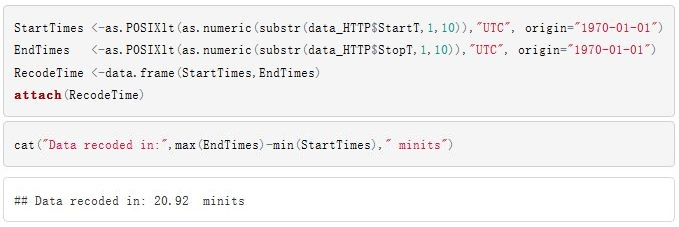
\includegraphics[width=15Cm]{images/lasttime}
\caption{Les données sont collectent dans 20.92 minutes}
\label{fig:lasttime}
\end{figure}

\subsection{Prétraitement de données}
En analysant des données, nous avons trouvé des erreurs de données, et le fournisseur nous a confirmé que ces sont les défaut de leur système 4G. Pour les attributs 'IMSI', 'IMEI', 'MSISDN', $90$ \% de lignes sont vides, ce qui ne sont pas vides, les contenus sont illisible, et peuvent provoquant des erreurs de lecture \ref{fig:errorData}. Et nous avons trouvé que dans les contenus de certains lignes sont bizarre. 
\begin{figure}[H]
	\centering
	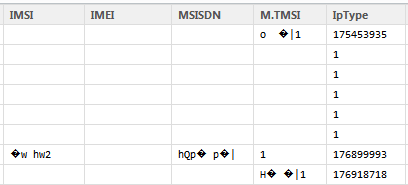
\includegraphics[width=0.7\linewidth]{images/errorData}
	\caption{erreur du codage BCD}
	\label{fig:errorData}
\end{figure}
Dans ce processus, le 'Down Link Online Time' égale à  $0$ ms , mais il a téléchargé $746$ bits, c'est clairement un erreur du données.
\begin{figure}[H]
	\centering
	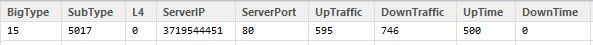
\includegraphics[width=0.9\linewidth]{images/bizarre}
	\caption{Erreur de la donnée}
	\label{fig:bizarre}
\end{figure}

 Nous avons décidé de ne utiliser les données avec ce type de erreur, à la fin, en supprimant ses données, il nous reste $37865$ lignes ($50894$ lignes en origine, $13029$ lignes ont été supprimé)  \ref{fig:newdata}.
 
\begin{figure}[H]
	\centering
	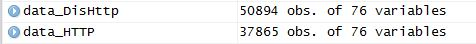
\includegraphics[width=0.8\linewidth]{images/newdata}
	\caption{Prétraitement des données}
	\label{fig:newdata}
\end{figure}

Dans certains lignes, il y a des erreurs de décompte. par exemple, dans un processus, il a téléchargé  $17$ paquets IP, et il a  $7448$  paquets sont désordre, et  ré-téléchargé  $6384$ paquets  \ref{fig:défaut}. Les données ne sont pas correct, donc nous ne pouvons pas utiliser ses donnée pour calculer les délai du service HTTP.  
\begin{figure}[H]
	\centering
	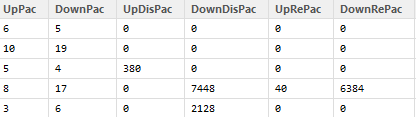
\includegraphics[width=0.7\linewidth]{images/11}
	\caption{Défaut de la système}
	\label{fig:défaut}
\end{figure}

\section{Solution existant}     
L'optimisation du service téléphonie est très important. L'opérateur a construit un immense réseau télécommunication, mais a cause de la mauvaise configuration du système, les utilisateur ne sont pas satisfais avec les services, les investissement n'a pas été remis. Donc les entreprises comme IBM, Huawei, et l'autre fournisseur du équipement essaient de trouver la meilleure solution. 

Maintenant, nous pouvons trouver beaucoup de papier sur l'optimisation du réseau télécommunication, mais les articles sont basé sur réseau 3G ou 2G, et la technique qu'ils utilisent ne sont pas convainquent. 

La technique utilise le plus souvent s'appelle 'KQI' ( Key Quality Indicator) \ref{fig:kqi}, cette méthode a été beaucoup utilisé. Et cette technique peut généralement divisé en deux étapes. d'abord, nous devons calculer le score de KPI, pour calcule le KPI en premier, il faut analyser le processus d'un service et choisir les indicateur de performances. Ensuite, nous pouvons calculer le score d'un processus en utilisant un équation linéaire, le poids de chaque attributs change selon le service, par exemple, pour le service SMS, le délai porte peu de l'importance, mais le délai du service est important pour le service HTTP. \textsf{à} la fin, nous pouvons calculer le KQI à avec les KPI \cite{kqi}. Mais les poids sont défini par les experts, et les valeurs peut-être fausse ou pas précis. Et par fois le score est bonne mais l'expérience de l'utilisateur n'est pas bon.
\begin{figure}[H]
\centering
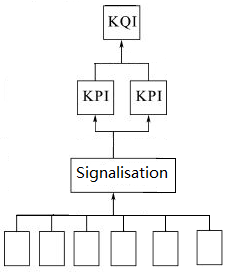
\includegraphics[width=5cm]{images/kqi}
\caption{KQI}
\label{fig:kqi}
\end{figure}

KPI est un des indicateurs de qualité axés sur les performances du réseau, mais il ne reflète pas directement l'expérience de la qualité de service de l'utilisateur, parce que les expériences de l'utilisateur sont difficile à mesure. Donc la technique QoE a été inventé. QoE défini la performance, de la qualité de service et l'expérience de l'utilisateur de l'ensemble du réseau à partir de l'utilisateur.

Les utilisateurs ont nombreuses exigences pour les services téléphonie, ils peuvent être résumées comme deux aspects: la fiabilité et le confort. La fiabilité fait référence à l'activité de l'accessibilité, la disponibilité et la durabilité. Le confort est une qualité de service, est un indice de la perception directe de l'utilisateur, qui dépend à l'expérience de l'utilisateur \cite{QoE}. Les relations entre QoE et QoS KPI sont: la fiabilité du service \ref{table.fiabilité}, le confort du service \ref{table.confort}. Maintenant, la technique de QoE a été beaucoup utilisé pour le service vocaux. Et a cause de la complexité des services de données, il n'y a pas un standard de QoE pour les services de données. 

\begin{table}[H]
	\centering
	\caption{Fiabilité du service }
	\label{table.fiabilité}
\begin{tabular}{|c|c|}
\hline \rule[-2ex]{0pt}{5.5ex} KQI & QoE \\ 
\hline \rule[-2ex]{0pt}{5.5ex} Accessibilité & Taux de succès  \\ 
\hline \rule[-2ex]{0pt}{5.5ex} Disponibilité  & Temps d'accès aux services \\ 
\hline \rule[-2ex]{0pt}{5.5ex} Durabilité & La durée de l'accès des services \\ 
\hline 
\end{tabular} 
\end{table}

\begin{table}[H]
	\centering
	\caption{Confort du service}
	\label{table.confort}
\begin{tabular}{|>{\centering\arraybackslash}p{5 cm}|>{\centering\arraybackslash}p{6 cm}|}
\hline KQI & QoE \\ 
\hline  & Taux de perte de paquets de couche d'application \\ 
\hline  & Le débit moyen  \newline \\ 
\hline La qualité du service de transmission & Stabilité de la transmission \\ 
\hline & Le bout en bout délai moyen \newline  \\ 
\hline & Gigue \newline  \\ 
\hline Le persistant de la connexion de service & La vitesse et la difficulté du service d'assistance\\ 
\hline 
\end{tabular} 
\end{table}

En utilisant la technique KQI et QoE, nous peuvent mesurer la qualité des différents services, les résultats peuvent aider les opérateurs trouver les services de mauvaise qualité, les opérateur peuvent améliorer les services selon le résultat, finalement améliorer la notation de l'utilisateur.  

Le résultat de KQI dépend seulement aux performances du réseau, donc nous avons besoin les informations des performances de réseau. Et la technologie QoE besoin Le résultat de KQI et les feed-back de l'utilisateur, le feed-back peut obtenir par l'enquête ou les plaintes des utilisateurs,  et par les mesures directs.

Aussi il y a un groupe qui utilise le comportement de l'utilisateur pour défini la qualité du service\cite{UB}. Le groupe utilise cette méthode dans le service vocaux, il cherche le situation comme l'utilisateur accroche et ré-appel le même personne. \textsc{à} la fin, cette méthode aide l'opérateur corriger le paramètre d'erreur.

Selon l'article le cette méthode peut aider l'opérateur trouver les défaut du système, mais il aa nombreuses restrictions, par exemple, nous ne pouvons pas utiliser cette technologie dans le service de SMS, etc.

\subsection{Notre solution}

La méthode qui utilise le comportement de l'utilisateur est intéressant, mais nous trouvons qu'elle peut utiliser seulement dans le service vocaux, nous n'avons pas trouvé les règles similaire dans l'autre service. D'ailleurs, le réseau LTE ne support pas le service vocaux, donc il n'existe pas optimisation du service vocaux dans réseau LTE et nous n'avons pas de données. Donc nous ne pouvons pas utiliser cette méthode.

La technique QoE et KQI sont beaucoup utilisé, mais d'abord, pour la méthode QoE, nous avons besoin les réponses des utilisateurs, mais nous n'avons pas assez de temps, et des raisons financières, CMCC ne peut pas nous fournir ces données. Et le équation qu'on utilise pour calcule KPI ne sont pas convaincante, voici un exemple d'un équation pour calcule la disponibilité du réseau\ref{fig:kpi}. 
\begin{figure}[H]
\centering
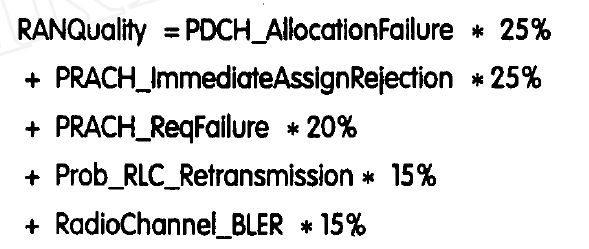
\includegraphics[width=0.7\linewidth]{images/kpi}
\caption{Un exemple d'un équation pour calculer la disponibilité}
\label{fig:kpi}
\end{figure}

Le poids du chaque attributs sont définir par les experts, Mais l'utilisateur n'est pas satisfaits du service. Nous croyons que l'erreur a été causée par l'inexacte équation, et nous pensons que les algorithmes de Classification peuvent aider à améliorer le résultat, mais très vite nous avons trouver que CMCC ne peut pas nous fournir ce type de données. Sans le connaissance a priori, nous ne pouvons pas utiliser ces algorithmes. Nous avons aussi pense à utiliser le externalisation ouverte (crowdsourcing), à notre avis si CMCC peut lancer un projet de externalisation ouverte, si CMCC peut encourager ses utilisateurs donnent les note aux services pour obtenir des crédits, nous pouvons obtenir les connaissance a priori, et a l'aide de ces données, nous pouvons trouver une équation peut-être mieux que les équations écrivent par les experts. Mais bien sur, CMCC n'a pas accepté cette idée, parce que cette méthode peut coûter cher, et il n'peut pas garantir le revenu. Et l'entreprise ne fait pas de l'investissement sans retour.

Finalement, nous avons décidé d'utiliser l'algorithme de clustering. C'est une méthodes statistiques d'analyse des données. Elle divise un ensemble de données en différents groupe, les données de chaque groupe ont mathématiquement plus proche que les données de l'autre groupe,  et on pense que les données dans le même sous-ensemble ont des caractéristique similaires.
\subsubsection{K-Means}
L'algorithme peut être divisé en 'clustering hiérarchiques' et 'clustering de partition'. Dans notre cas, nous avons utiliser l'algorithme K-Means. 

Le but de cet algorithme est de diviser des données en K partitions (clusters) dans lesquelles les données appartient à la partition avec la moyenne la plus proche. C'est une méthode classique, il a été utilisés dans beaucoup différents domaines.

q
\subsubsection{Algorithme règles}
Après avoir utilisé le K-Means, nous pouvons utiliser le algorithme règles d'association pour trouver des règles qui peuvent nous aider à faire la décision.


















  \cleardoublepage
    
  \section{La première section}


\subsection{Une sous section}

On peut mettre des mots en \emph{italique}, 
en \textsc{petites Majuscules} ou 
en \texttt{largeur fixe (machine à écrire)}.

Voici un deuxième paragraphe avec une formule mathématique simple : $e = mc^2$.

Un troisième avec des \og guillemet français \fg{}.

\subsubsection{Écrire en anglais}

\foreignlanguage{english}{Do you speak French? Does anybody here speak french?}


\subsection{Lites}

\begin{itemize}
\item Liste classique ;
\item un élément ;
\item et un autre élément.
\end{itemize}
\vspace{\parskip} % espace entre paragraphes

\begin{enumerate}
\item Une liste numéroté
\item deux
\item trois
\end{enumerate}
\vspace{\parskip}

\begin{description}
\item[Description] C'est bien pour des définitions.
\item[Deux] Ou pour faire un liste spéciale.
\end{description}
\vspace{\parskip}


\subsection{Références}

Voici une référence à l'image de la figure \ref{bloghiko} page \pageref{bloghiko} et une autre vers la partie \ref{p2} page \pageref{p2}.

On peut citer un livre\,\up{\cite{lpp}} et on précise les détails à la fin du rapport dans la partie références.


\subsection{Note de bas de page}

Voici une note\,\footnote{Texte de bas de page} de bas de page.
Une deuxième\,\footnotemark{} déclarée différemment.
La même note\,\footnotemark[\value{footnote}].

\footnotetext{Il a deux références vers cette note}


\subsection{Figure}

\begin{figure}[!ht]
    \center
    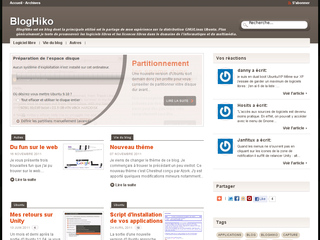
\includegraphics[]{./images/bloghiko.jpg}
    \caption{BlogHiko | taille original}
    \label{bloghiko}
\end{figure}

\begin{figure}[H]
    \center
    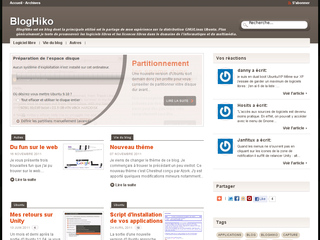
\includegraphics[width=0.5\textwidth]{./images/bloghiko.jpg}
    \caption{BlogHiko | 50\% de la largeur de la page}
\end{figure}



  \cleardoublepage
  
  \section{Citation Wikipédia}
\label{p2}


LaTeX est un langage et un système de composition de documents créé par Leslie Lamport en 198312. Plus exactement, il s'agit d'une collection de macro-commandes destinées à faciliter l'utilisation du \og processeur de texte \fg{} TeX de Donald Knuth. Depuis 1993, il est maintenu par le LaTeX3 Project team. La première version utilisée largement, appelée LaTeX2.09, est sortie en 1984. Une révision majeure, appelée LaTeX2 epsilon est sortie en 1991.

Le nom est l'abréviation de Lamport TeX. On écrit souvent \LaTeX, le logiciel permettant les mises en forme correspondant au logo.

Du fait de sa relative simplicité, il est devenu la méthode privilégiée d'écriture de documents scientifiques employant TeX. Il est particulièrement utilisé dans les domaines techniques et scientifiques pour la production de documents de taille moyenne ou importante (thèse ou livre, par exemple). Néanmoins, il peut aussi être employé pour générer des documents de types variés (par exemple, des lettres, ou des transparents).


  \cleardoublepage
  
  \section*{Conclusion}
\addcontentsline{toc}{section}{Conclusion}

Pendant ce 4 mois de stage, nous avons lu beaucoup de articles, nous avons préparé des dossier et fait des rapport pour le CMCC, aussi nous avons négocié avec les gens du CMCC et les gens du fournisseur de l'équipement. Nous avons perdu beaucoup de temps en négocier et attendre, mais finalement, nous avons trouvé 2 méthode pour résoudre le problème du CMCC.

Dans le rapport, j'ai présenté les algorithmes et la mise en \oe uvre, mais malheureusement, les résultats ne sont pas satisfaisant, nous avons essayé différent paramètre, différente technique, différent logiciel, mais nous n'avons pas trouvé un résultat satisfaisant. Donc nous croyons que cela est causée du fait que la qualité de données est mal. Et parce que nous avons seulement le données erronées, nous ne pouvons pas évaluer notre techniques.

Cependant, pour l'entreprise CMCC, nous avons fait une démonstration en comment utilise les technique de fouille de données avec ses données, et les inconvénients de son système. Et aussi nous montrons que si il a le données non erronées, comme il peut trouver les informations qu'il a besoin.

Pour moi, j'ai utilisé différente algorithme et les logiciel, et j'ai utilisé le langage R pour résoudre les problème. 

J'ai rencontré des bons amis dans le laboratoire, et j'ai acquis des expérience professionnel.

\newpage
\section*{Les travaux futurs}





  \cleardoublepage
  
  \phantomsection\addcontentsline{toc}{section}{Références}
\begin{thebibliography}{ABC}	
    %\bibitem[REF]{reference} auteur. \emph{titre}. édition, année.

    
    \bibitem[1]{specifi}R\&D \textsc{département de }CMCC.   \emph{Interface Specification of China Mobile Signaling Monitoring System(LTE Signal Collection Gateway Part)}.
    \bibitem[2]{kqi}Jianhua DU, Shiwen LU, Fangfeng ZHANG  \emph{Research of KQI Development Methodology in SQM},2008.
    \bibitem[3]{QoE}Luning ZHAO, Zhuo SUN, Wenbo WANG  \emph{Mobile streaming QoE index system and quantify},2012.
    \bibitem[4]{UB} Rui WANG, Fei SU, Zhengdong HAN, Zilong CAI. \emph{The Recessive Problem Mining and Optimization Research of Voice Service Based on User Behaviors}. édition, 2013.
    \bibitem[5]{SC} Lianjiang ZHU, Bingxian MA, Xuequan ZHAO. \emph{Clustering validity analysis based on silhouette coefficient}, 2010.
     \bibitem[6]{AR} Hongyan WANG, Daiwen WU. \emph{Discussion on digging algorithm of correlation rule for numerical attribute}, 2012.
     \bibitem[7]{KmMst}Hao OUYANG, Bo CHEN, Zhenjin HUANG, Meng WANG, Zhiwen WANG. \emph{MST Clustering Algorithme Based on K-Means}. 2014.
\end{thebibliography}

%
\end{document}

